\documentclass[aspectratio=169,11pt]{beamer}

\usetheme{default}
\usepackage[T1]{fontenc}
\usepackage[utf8]{inputenc}
\usepackage{lmodern}
\usepackage{graphicx}

\setbeamertemplate{navigation symbols}{}
\setbeamertemplate{section in toc}[sections numbered]
\setbeamertemplate{footline}{%
  \leavevmode%
  \hbox{%
    \begin{beamercolorbox}[
      wd=0.86\paperwidth,
      ht=2.6ex,
      dp=1.0ex,
      leftskip=0.5cm
    ]{author in head/foot}%
      \insertsectionnumber. \insertsectionhead
    \end{beamercolorbox}%
    \begin{beamercolorbox}[
      wd=0.14\paperwidth,
      ht=2.6ex,
      dp=1.0ex,
      center
    ]{date in head/foot}%
      \insertframenumber/\inserttotalframenumber
    \end{beamercolorbox}%
  }%
}

\graphicspath{{figures/}}

\title{Final Project}
\subtitle{Airbnb Price Prediction in Tokyo}
\author{Jakob Kauws}
\date{Machine Learning, SoSe 2026}

\AtBeginSection[]{%
  \begin{frame}[plain]
    \vfill
    \centering
    {\usebeamerfont{title}%
      \usebeamercolor[fg]{structure}%
      \insertsectionnumber.\ \insertsectionhead\par}
    \vfill
  \end{frame}
}

\begin{document}

\begin{frame}[plain]
  \titlepage
\end{frame}

\begin{frame}[plain]{Contents}
  \tableofcontents
\end{frame}

\section{Data Cleaning and Preparation}

\begin{frame}{1.1 Data}
  \begin{itemize}
    \item City: Tokyo
    \item Inside Airbnb snapshot: September 2025
    \item Raw data: 27,945 listings
    \item Files: listings, reviews, images
    \item Modalities: tabular, spatial, text, images
    \item Target: nightly asking price
  \end{itemize}
\end{frame}

\begin{frame}{1.2 Price Distribution}
  \centering
  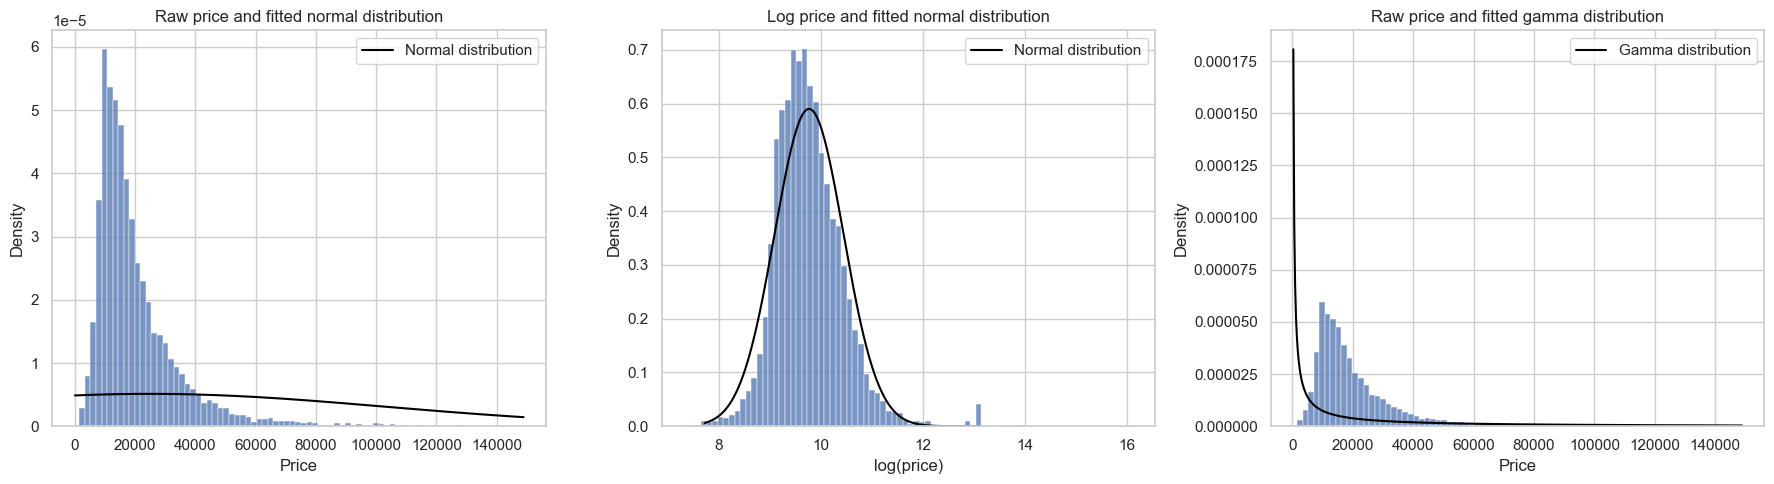
\includegraphics[
    width=\textwidth,
    height=0.78\textheight,
    keepaspectratio
  ]{target_distributions.png}
\end{frame}

\begin{frame}{1.3 Data Preparation}
  \begin{itemize}
    \item Price cleaning
    \item Number of positive prices: 25,480
    \item Mean price: 24,782 JPY
    \item Median price: 16,200 JPY
    \item Log transformation
    \item Train-test split: 80/20
  \end{itemize}
\end{frame}

\section{Feature Engineering}

\begin{frame}{2.1 Tabular Features}
  \begin{columns}[T,onlytextwidth]
    \begin{column}{0.47\textwidth}
      \textbf{Numeric features}
      \begin{itemize}
        \item Median imputation
        \item Log transforms
        \item Standardization
      \end{itemize}
    \end{column}
    \begin{column}{0.47\textwidth}
      \textbf{Categorical features}
      \begin{itemize}
        \item Missing categories
        \item One-hot encoding
        \item Review-score buckets
        \item Amenity indicators: 21
      \end{itemize}
    \end{column}
  \end{columns}
\end{frame}

\begin{frame}{2.2 Spatial Features and Interactions}
  \begin{itemize}
    \item Latitude and longitude splines
    \item Neighbourhood $\times$ room type
    \item Property group $\times$ accommodates
    \item Amenities $\times$ property group
    \item Review score $\times$ review count
    \item Final matrix: 1,017 features
  \end{itemize}
\end{frame}

\begin{frame}{2.3 Text Features}
  \begin{itemize}
    \item Listing text: title, description, neighbourhood overview, host profile
    \item Review text: 10 latest reviews
    \item Amenities: text representation
    \item Native CatBoost text
    \item Word and character TF-IDF
    \item Truncated SVD: 128 features
  \end{itemize}
\end{frame}

\begin{frame}{2.4 Image Features}
  \begin{columns}[T,onlytextwidth]
    \begin{column}{0.47\textwidth}
      \textbf{Transformation}
      \begin{itemize}
        \item Main listing image
        \item CLIP image embedding
        \item Similarity to 15 prompts
      \end{itemize}
    \end{column}
    \begin{column}{0.47\textwidth}
      \textbf{Model features}
      \begin{itemize}
        \item 15 similarity scores
        \item Image availability indicator
      \end{itemize}
    \end{column}
  \end{columns}
\end{frame}

\section{Modeling and Tuning}

\begin{frame}{3.1 Linear Regression}
  \begin{columns}[T,onlytextwidth]
    \begin{column}{0.47\textwidth}
      \textbf{Input}
      \begin{itemize}
        \item Tabular features
        \item Spatial features
      \end{itemize}
    \end{column}
    \begin{column}{0.47\textwidth}
      \textbf{Results}
      \begin{itemize}
        \item Log-price MSE: 0.202
        \item Log-price $R^2$: 0.550
        \item Price MAE: 8,960 JPY
        \item Median AE: 3,387 JPY
      \end{itemize}
    \end{column}
  \end{columns}
\end{frame}

\begin{frame}{3.2 Group-wise Linear Boosting}
  \centering
  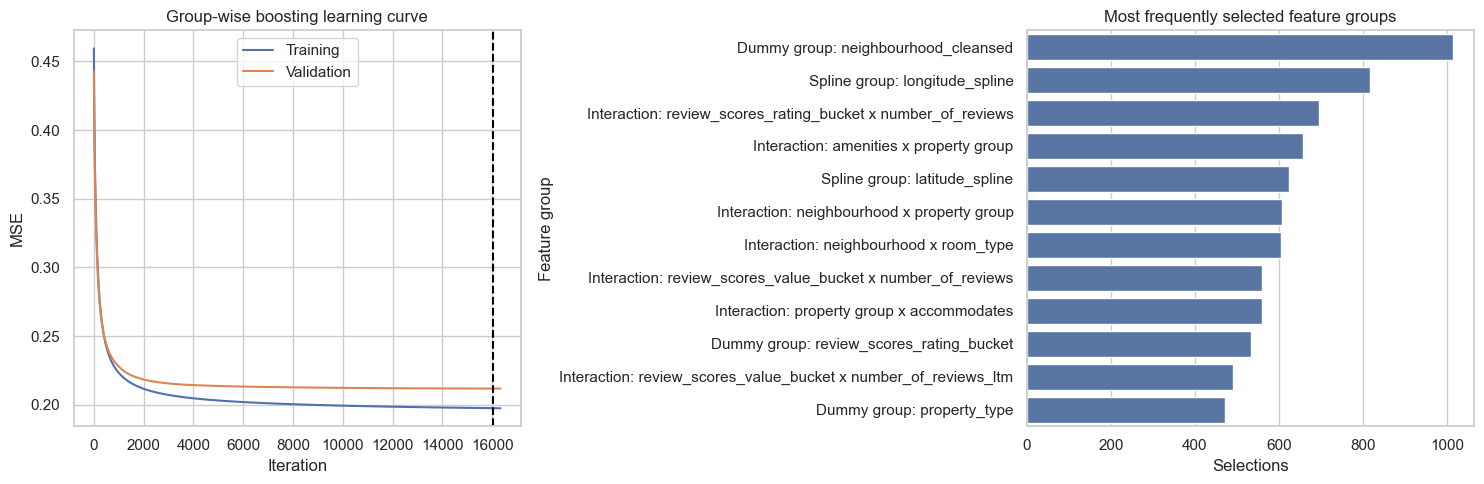
\includegraphics[
    width=\textwidth,
    height=0.78\textheight,
    keepaspectratio
  ]{groupwise_boosting.png}
\end{frame}

\begin{frame}{3.2 Group-wise Linear Boosting}
  \begin{columns}[T,onlytextwidth]
    \begin{column}{0.47\textwidth}
      \textbf{Input}
      \begin{itemize}
        \item Tabular features
        \item Spatial features
      \end{itemize}
    \end{column}
    \begin{column}{0.47\textwidth}
      \textbf{Results}
      \begin{itemize}
        \item Log-price MSE: 0.198
        \item Log-price $R^2$: 0.558
        \item Price MAE: 8,941 JPY
        \item Median AE: 3,458 JPY
      \end{itemize}
    \end{column}
  \end{columns}
\end{frame}

\begin{frame}{3.3 Histogram Gradient Boosting}
  \begin{columns}[T,onlytextwidth]
    \begin{column}{0.47\textwidth}
      \textbf{Input}
      \begin{itemize}
        \item Tabular features
        \item Spatial features
      \end{itemize}
    \end{column}
    \begin{column}{0.47\textwidth}
      \textbf{Results}
      \begin{itemize}
        \item Log-price MSE: 0.142
        \item Log-price $R^2$: 0.683
        \item Price MAE: 8,010 JPY
        \item Median AE: 2,765 JPY
      \end{itemize}
    \end{column}
  \end{columns}
\end{frame}

\begin{frame}{3.4 CatBoost: Tabular Data}
  \begin{columns}[T,onlytextwidth]
    \begin{column}{0.47\textwidth}
      \textbf{Input}
      \begin{itemize}
        \item Tabular features
        \item Spatial features
      \end{itemize}
    \end{column}
    \begin{column}{0.47\textwidth}
      \textbf{Results}
      \begin{itemize}
        \item Log-price MSE: 0.117
        \item Log-price $R^2$: 0.739
        \item Price MAE: 6,904 JPY
        \item Median AE: 2,382 JPY
      \end{itemize}
    \end{column}
  \end{columns}
\end{frame}

\begin{frame}{3.5 CatBoost: TF-IDF reduced with SVD}
  \begin{columns}[T,onlytextwidth]
    \begin{column}{0.47\textwidth}
      \textbf{Input}
      \begin{itemize}
        \item Tabular features
        \item Spatial features
        \item TF-IDF reduced with SVD
      \end{itemize}
    \end{column}
    \begin{column}{0.47\textwidth}
      \textbf{Results}
      \begin{itemize}
        \item Log-price MSE: 0.113
        \item Log-price $R^2$: 0.748
        \item Price MAE: 6,293 JPY
        \item Median AE: 2,377 JPY
      \end{itemize}
    \end{column}
  \end{columns}
\end{frame}

\begin{frame}{3.6 CatBoost: Native Text}
  \begin{columns}[T,onlytextwidth]
    \begin{column}{0.47\textwidth}
      \textbf{Input}
      \begin{itemize}
        \item Tabular features
        \item Spatial features
        \item Native text features
      \end{itemize}
    \end{column}
    \begin{column}{0.47\textwidth}
      \textbf{Results}
      \begin{itemize}
        \item Log-price MSE: 0.105
        \item Log-price $R^2$: 0.766
        \item Price MAE: 6,230 JPY
        \item Median AE: 2,159 JPY
      \end{itemize}
    \end{column}
  \end{columns}
\end{frame}

\begin{frame}{3.7 CatBoost: Native Text and CLIP}
  \begin{columns}[T,onlytextwidth]
    \begin{column}{0.47\textwidth}
      \textbf{Input}
      \begin{itemize}
        \item Tabular features
        \item Spatial features
        \item Native text features
        \item CLIP prompt features
      \end{itemize}
    \end{column}
    \begin{column}{0.47\textwidth}
      \textbf{Results}
      \begin{itemize}
        \item Log-price MSE: 0.105
        \item Log-price $R^2$: 0.765
        \item Price MAE: 6,239 JPY
        \item Median AE: 2,202 JPY
      \end{itemize}
    \end{column}
  \end{columns}
\end{frame}

\begin{frame}{3.8 CatBoost: Native Text and CLIP, Long Run}
  \begin{columns}[T,onlytextwidth]
    \begin{column}{0.47\textwidth}
      \textbf{Input}
      \begin{itemize}
        \item Tabular features
        \item Spatial features
        \item Native text features
        \item CLIP prompt features
      \end{itemize}
    \end{column}
    \begin{column}{0.47\textwidth}
      \textbf{Results}
      \begin{itemize}
        \item Log-price MSE: 0.102
        \item Log-price $R^2$: 0.772
        \item Price MAE: 6,053 JPY
        \item Median AE: 2,133 JPY
      \end{itemize}
    \end{column}
  \end{columns}
\end{frame}

\begin{frame}{3.9 CatBoost: Native Text, Long Run}
  \begin{columns}[T,onlytextwidth]
    \begin{column}{0.47\textwidth}
      \textbf{Input}
      \begin{itemize}
        \item Tabular features
        \item Spatial features
        \item Native text features
      \end{itemize}
    \end{column}
    \begin{column}{0.47\textwidth}
      \textbf{Results}
      \begin{itemize}
        \item Log-price MSE: 0.103
        \item Log-price $R^2$: 0.770
        \item Price MAE: 5,929 JPY
        \item Median AE: 2,081 JPY
      \end{itemize}
    \end{column}
  \end{columns}
\end{frame}

\section{Analysis and Reporting}

\begin{frame}{4.1 Model Comparison}
  \centering
  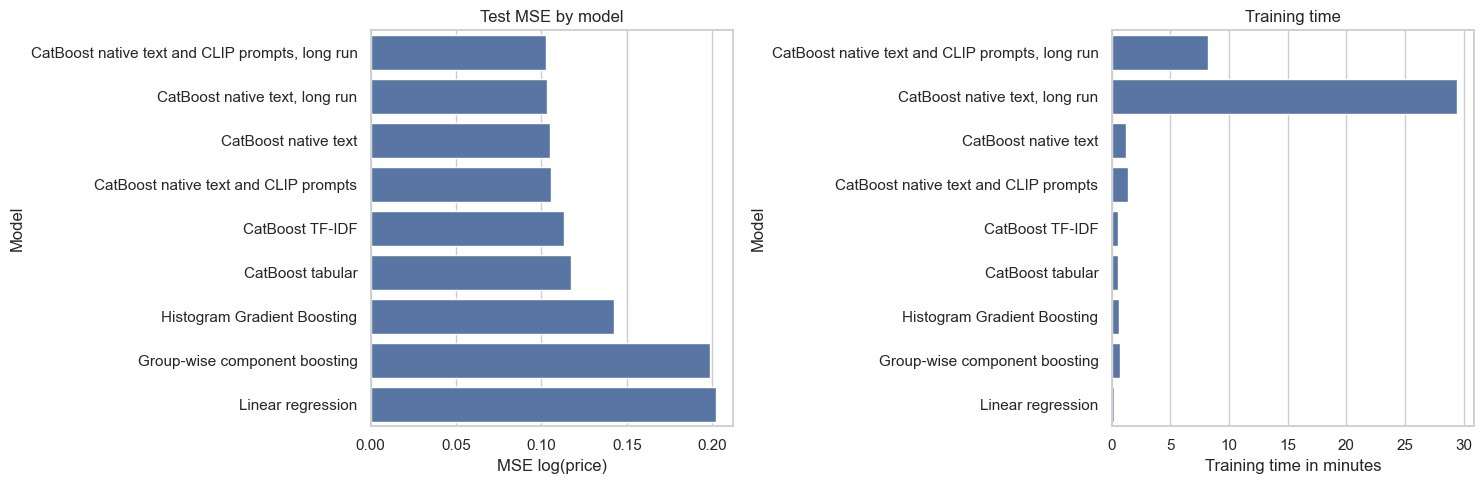
\includegraphics[
    width=\textwidth,
    height=0.78\textheight,
    keepaspectratio
  ]{model_comparison.png}
\end{frame}

\begin{frame}{4.1 Main Results}
  \begin{itemize}
    \item Best log-price MSE: Native text and CLIP, long run
    \item Lowest price MAE: Native text, long run
    \item Main improvement: text features
    \item No clear improvement: image features
  \end{itemize}
\end{frame}

\begin{frame}{4.2 Predictions and Residuals}
  \centering
  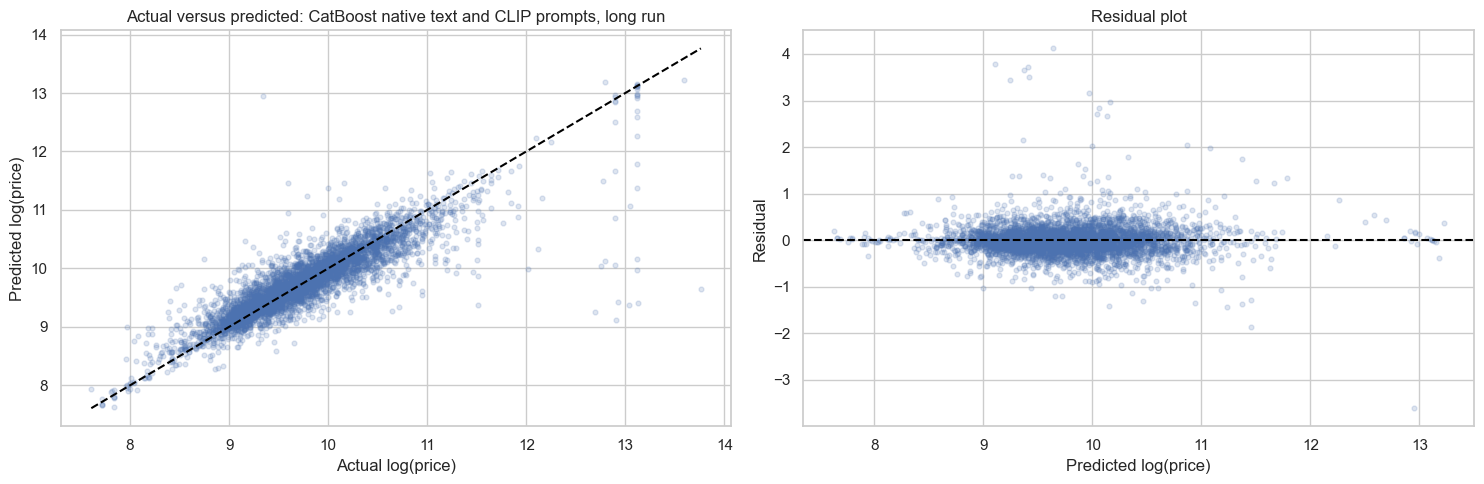
\includegraphics[
    width=\textwidth,
    height=0.78\textheight,
    keepaspectratio
  ]{prediction_residuals.png}
\end{frame}

\begin{frame}{4.3 Feature Importance}
  \centering
  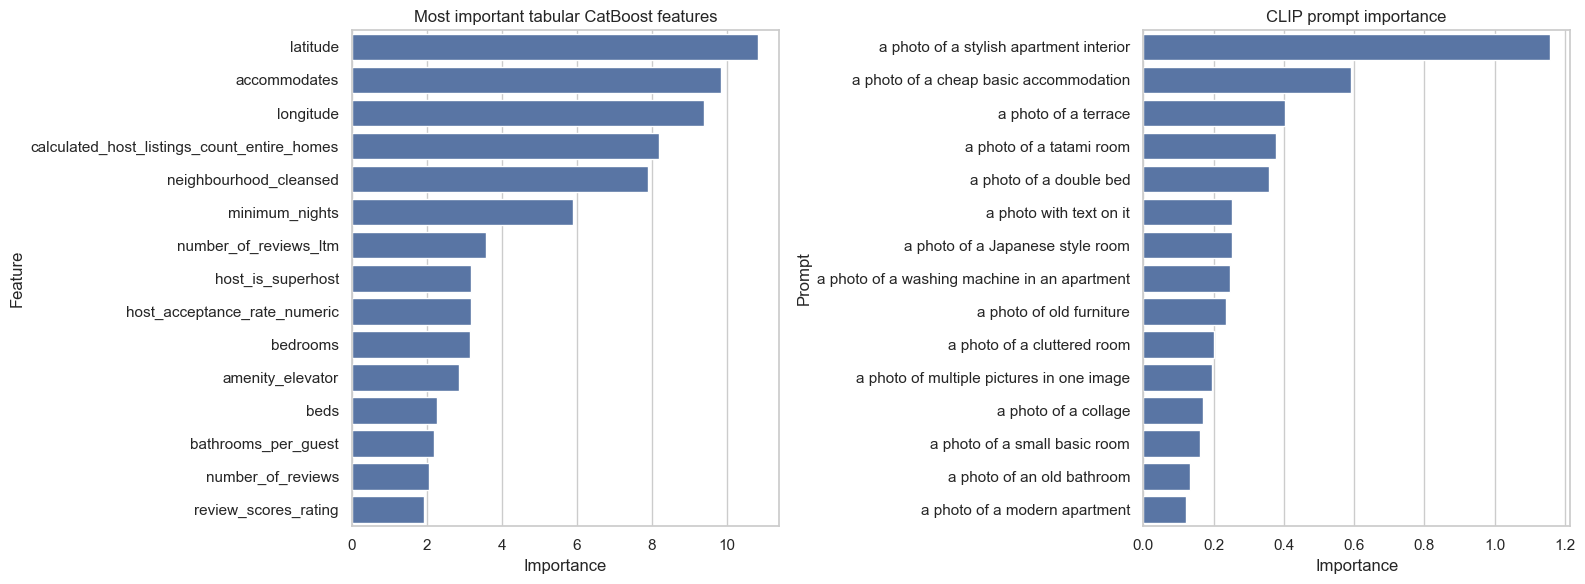
\includegraphics[
    width=\textwidth,
    height=0.78\textheight,
    keepaspectratio
  ]{feature_importance.png}
\end{frame}

\begin{frame}{4.3 Main Features}
  \begin{itemize}
    \item Location
    \item Capacity
    \item Host activity
    \item Minimum nights
  \end{itemize}
\end{frame}

\begin{frame}{4.4 Limitations}
  \begin{itemize}
    \item Asking prices
    \item Single point-in-time snapshot
    \item Extreme round prices
    \item Missing reviews: new listings
    \item Repeated images and descriptions: same host
  \end{itemize}
\end{frame}

\end{document}
